\section{Robotic arm Kinematic Analysis}


\subsection{Robotic arm, DH parameters \& Forward Kinematics}

\begin{center}
\begin{figure}[H]
\centering
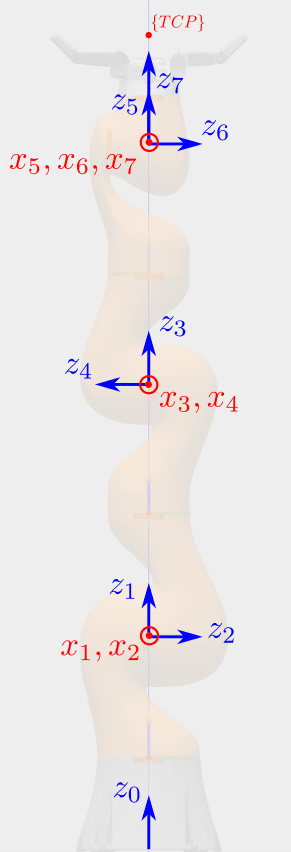
\includegraphics[height=12cm]{images/iiwa-frames.png}\\
\caption{Joint reference frames of the KUKA iiwa14 robot}
\end{figure}
\end{center}

\begin{center}
\begin{tabular}{ |c|c|c|c|c| } 
\hline
i & $θ_i$ (rad) & $L_{i-1}$ (m) & $d_i$ (m) & $α_{i-1}$ (rad) \\
\hline
1 & $θ_1$ & 0 & 0.36 & 0 \\
2 & $θ_2$ & 0 & 0 & $-π/2$ \\
3 & $θ_3$ & 0 & 0.36 & $π/2$ \\
4 & $θ_4$ & 0 & 0 & $π/2$\\
5 & $θ_5$ & 0 & 0.4 & $-π/2$ \\
6 & $θ_6$ & 0 & 0 & $-π/2$ \\
7 & $θ_7$ & 0 & 0 & $π/2$ \\
\hline
\end{tabular}
\end{center}

\[
^{i-1}T_i = 
\begin{bmatrix}
c\theta_i & -s\theta_i & 0 & L_{i-1} \\
s\theta_ica_{i-1} & c\theta_ica_{i-1} & -sa_{i-1} & -sa_{i-1}d_i \\
s\theta_isa_{i-1} & c\theta_isa_{i-1} & ca_{i-1} & ca_{i-1}d_i \\
0 & 0 & 0 & 1\\
\end{bmatrix}
\]


\subsection{Inverse Kinematics}

\subsubsection{Decoupling Technique}

In this section the inverse kinematics problem is solved for only the 6 out of the 7 total degrees of freedom. The third joint is not used in this 
analysis and it's angle is set to zero $θ_3 = 0$ . The rest of the joints form a special kind of kinematic chain that can be solved using the 
decoupling technique. In this technique the Inverse kinematics problem is split to 2 separate subproblems, one for the position and one for the 
orientation of the end-effector. This technique can be applied in this case because the axes of the 3 last joints intersect at the same point and 
they form an Euler wrist. \\

To solve for the joints' angles, the transformation matrix $^0T_7$ of the end-effector with respect to the robot's base is required. Usually the transformation ${}^UT_{tcp}$ is known, which is the pose of Tool's center point (TCP) with respect to the Universal Coordinate Frame $\lbrace U \rbrace$ from which the required $^0T_7$ can be calculated

\[
{}^UT_{tcp} = {}^UT_0  \;\;  {}^0T_7  \;\;   {}^7T_{tcp}
\]
\[
{}^0T_7 = {}^UT_0^{-1}  \;\;  {}^UT_{tcp}  \;\;  {}^7T_{tcp}^{-1}
\]
\[
{}^0T_7 = \begin{bmatrix}
R_t & \mathbf{p}_t \\
0 & 1 \\
\end{bmatrix}
\]

where ${}^UT_0,  \;\;   {}^7T_{tcp}$ are translation transformations by a constant distance and $R_t,  \;\; \mathbf{p}_t$ are the target's orientation 
and position respectively.

\[
{}^0\mathbf{p}_5 = {}^0T_4 {}^4\mathbf{p}_5 = \begin{bmatrix} p_x \\ p_y \\ p_z \\ \end{bmatrix}
\]

\begin{equation}
θ_1 = 
\begin{cases}
atan2 \left( p_y, p_x \right) \\
π - atan2 \left( p_y, p_x \right)
\end{cases}
\end{equation}

\begin{center}
\begin{figure}[H]
\centering
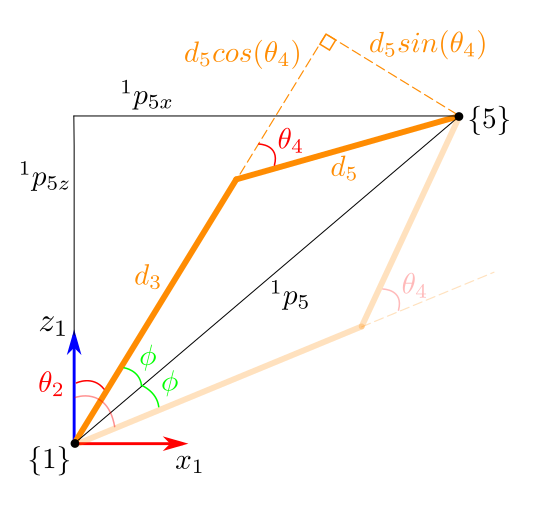
\includegraphics[width=8cm]{images/th2-4-calculation.png}\\
\caption{Calculation of angles $θ_2, θ_4$}
\end{figure}
\end{center}

\[
φ = acos \left( \frac{d_3^2 + \Vert{}^1p_{5}\Vert ^2 - d_5^2}{2d_3 \Vert{}^1p_{5}\Vert} \right)
\]
\begin{equation}
θ_2 = atan2 \left( \sqrt{p_x^2 + p_y^2}, {}^1p_{5z} \right) \pm φ
\end{equation}

\[ c_4 = \frac{ \Vert{}^1p_{5}\Vert ^2 - d_3^2 - d_5^2 }{2d_3d_5} \]
\begin{equation}
θ_4 = atan2 \left( \pm \sqrt{1 - c_4^2}, c_4 \right)
\end{equation}

Once $θ_1,θ_2,θ_3,θ_4$ are known, the orientation matrix of the wrist can be calculated as following
\[
R_{target} = 
\begin{bmatrix}
i_x & j_x & k_x\\
i_y & j_y & k_y\\
i_z & j_z & k_z\\
\end{bmatrix}
\]
\begin{equation}
θ_6 = atan2 \left( \pm \sqrt{1-k_y^2}, k_y \right)
\end{equation}
\[
θ_7 = atan2 \left( -j_y, i_y \right)
\]
\[
θ_5 = atan2 \left( - k_z, k_x \right)
\]


\subsubsection{Workspace constraints \& Singularity points}

\begin{center}
\begin{figure}[H]
\centering
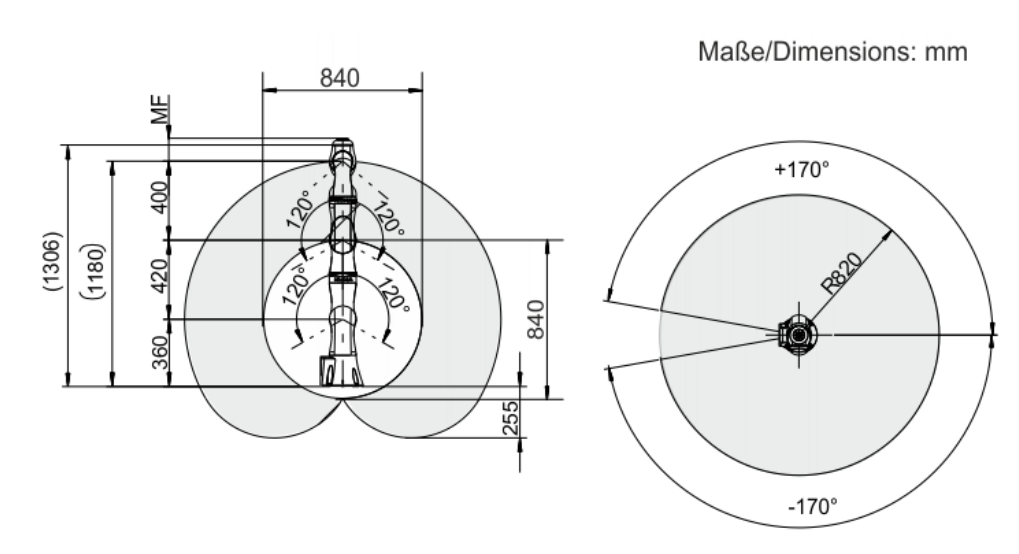
\includegraphics[width=10cm]{images/iiwa-workspace.png}\\
\caption{KUKA iiwa LBR14 workspace dimensions}
\end{figure}
\end{center}

Singularity points:
\begin{itemize}
	\item When $p_x^2 + p_y^2 = 0$ then the end-effector lies on the z-axis and $θ_1$ is not defined
	\item When $sin\left( θ_6 \right) = 0$ then the angles $θ_5, θ_7$ are not defined
\end{itemize}

\subsubsection{Solutions for 7DoF numerically}

\subsubsection{Comparison of Inverse Kinematics Techniques}
